\documentclass[conference]{IEEEtran}
\IEEEoverridecommandlockouts

\usepackage{cite}
\usepackage{amsmath,amssymb,amsfonts}
\usepackage{algorithmic}
\usepackage{graphicx}
\usepackage{textcomp}
\usepackage{xcolor}
\usepackage{booktabs}
\usepackage{multirow}
\usepackage{url}
\usepackage{hyperref}

\def\BibTeX{{\rm B\kern-.05em{\sc i\kern-.025em b}\kern-.08em
    T\kern-.1667em\lower.7ex\hbox{E}\kern-.125emX}}

\begin{document}

\title{Confidence-Driven Occlusion-Aware Camera--Radar Fusion for\\
Hidden Hazard Prediction in Autonomous Driving}

% ---------------------------------------------------------------------
% NOTE TO AUTHORS: replace the affiliation/department/city placeholders
% below with your institution's actual details before submission.
% ---------------------------------------------------------------------
\author{
\IEEEauthorblockN{Maddan M}
\IEEEauthorblockA{\textit{Department of Computer Science and Engineering} \\
\textit{[Your Institution Name]}\\
[City, Country] \\
[email address]}
\and
\IEEEauthorblockN{Sankkarshana N}
\IEEEauthorblockA{\textit{Department of Computer Science and Engineering} \\
\textit{[Your Institution Name]}\\
[City, Country] \\
[email address]}
}

\maketitle

\begin{abstract}
Advanced driver-assistance and autonomous-driving perception stacks are
usually evaluated on what they detect, not on what they fail to see. An
occluded pedestrian stepping out from behind a parked vehicle is one of
the most common and most dangerous scenarios in urban driving, yet most
camera--radar fusion pipelines have no explicit representation of
occlusion, no calibrated notion of detection confidence, and no way to
reason about a hazard that is momentarily invisible to every sensor.
This paper presents a nine-component perception framework, built and
evaluated entirely in the CARLA simulator, that starts from the opposite
premise: the system should \emph{quantify and explain what it cannot
see}. The framework combines an evidential (Dirichlet) confidence head
over a YOLOv8n detector, a three-state bird's-eye occlusion grid fused
from monocular depth and radar, a Bayesian contradiction resolver that
conditions sensor likelihoods on occlusion state, an extended Kalman
filter for visible-target tracking, a particle filter for
multi-hypothesis reasoning about fully occluded hazards, a
crossing-intent predictor, a dynamic risk-scoring engine, a
self-referential sensor health monitor, and an adversarial robustness
test harness. The system is evaluated on a 15{,}270-frame dataset
collected from a roaming, autopilot-driven ego vehicle across 170
episodes in CARLA 0.10.0's Town10HD\_Opt. The evidential classifier
reaches $96.2\% \pm 0.8\%$ validation accuracy on a split grouped by
episode rather than by crop, with uncertainty that is empirically
calibrated against true error. Camera--radar fusion reduces
lateral-velocity estimation error by 18\% relative to camera alone and
60\% relative to radar alone on paired observations, and improves
crossing-intent prediction F1 from 0.733 (camera-only) to 0.855
(fused). The occlusion detector, after a ground-truth camera-projection
defect was found, proven, and fixed, and after a subsequent fix to a
disparity-quantile estimator that turned out to be the real recall
bottleneck, recovers a recall of 0.917 at a precision of 0.727. Explicit
adversarial testing shows the sensor health monitor detecting five of
seven injected fault classes; the remaining two, radar range bias and
sustained radar clutter, are shown to be structurally difficult for any
self-referential monitor to catch, and we report that limitation rather
than talk around it. We argue that this kind of end-to-end,
adversarially-tested, uncertainty-aware architecture, together with the
discipline of validating ground truth independently of the system under
test, is a necessary complement to accuracy-only benchmarking for
safety-critical perception.
\end{abstract}

\begin{IEEEkeywords}
autonomous driving, sensor fusion, occlusion-aware perception, evidential deep
learning, uncertainty quantification, particle filter, extended Kalman filter,
pedestrian crossing intent, CARLA simulation, sensor health monitoring
\end{IEEEkeywords}

\section{Introduction}

Urban autonomous driving is dominated by a class of failure that
occupancy-grid and bounding-box benchmarks tend to under-represent: the
hazard that is not currently visible. A pedestrian stepping out from
behind a parked bus, a cyclist emerging from a blind driveway, a child
crossing between two vehicles: in all of these, the presence and
trajectory of the hazard is, for a window of time, unavailable to every
onboard sensor. A perception stack that only reports what it currently
detects has nothing useful to say about that window. The premise of
this work is that a safety-relevant perception system has to represent
what it cannot see: which regions of the scene are occluded, how
confident it is in the detections it does have, and what it should
believe about a hazard that has gone temporarily invisible.

That premise has three concrete consequences for the system described
in this paper. First, detection confidence has to be a first-class,
calibrated quantity rather than a bare classifier score, so we use an
evidential (Dirichlet) confidence head that raises uncertainty
predictably on ambiguous or partially-visible detections. Second,
occlusion has to be modelled explicitly, as a three-state
(visible/occluded/empty) bird's-eye grid built from sensor data alone
and never from privileged simulator state, so the same inference works
in principle on a real vehicle. Third, once a tracked target becomes
fully occluded, its future position is not a single point estimate.
It may continue on its original heading, slow down, stop, or reverse,
and that is a genuinely multi-modal distribution that a Kalman filter's
unimodal Gaussian cannot represent but a particle filter can.

Beyond the perception pipeline itself, this paper leans hard on two
forms of validation that simulation-based ADAS research tends to skip:
adversarial fault injection against the system's own self-monitoring,
and independent verification of the \emph{ground truth} the system is
scored against. The second point mattered in a very concrete way,
described in Section~\ref{sec:results}. A sign error in
the camera projection used to generate occlusion ground truth caused
every occlusion-detector metric to validate against itself for two full
data-collection cycles before anyone found it, because the same
projection code was shared, by design, between the ground-truth
generator and part of the runtime system. We report this defect, its
proof, and its correction in full, because the lesson generalises well
beyond this project: ground truth has to be independently verifiable,
not just internally consistent.

The contributions of this paper are:
\begin{itemize}
\item A nine-component, occlusion-aware perception architecture
  combining evidential confidence estimation, monocular-depth-plus-radar
  occlusion sensing, occlusion-conditioned Bayesian sensor fusion,
  dual-mode (Kalman/particle) tracking, crossing-intent prediction,
  dynamic risk scoring, and a self-referential sensor health monitor,
  implemented and evaluated end to end in CARLA.
\item A 15{,}270-frame dataset collected from a continuously-driving,
  autopilot-controlled ego vehicle that actively encounters staged
  occlusions in live urban traffic, together with the specific,
  measured defects found in an earlier 8{,}280-frame pilot collection
  (deleted fully-occluded ground truth, geometrically guaranteed-empty
  scenario frames, and a non-functional simulator weather API) and the
  fixes applied.
\item Quantitative sensor-fusion, crossing-intent, and occlusion-detection
  results, reported on paired (identically-observed) subsets rather
  than aggregate means. We show the two can produce opposite
  conclusions, which is reason enough not to trust the aggregate.
\item An adversarial robustness evaluation that explicitly tests
  whether the system's own health monitor notices seven injected
  sensor faults, plus a detailed account of two faults, sustained
  radar clutter and radar range bias, that a self-referential monitor
  cannot structurally detect, including a fix attempt that was tried,
  measured, found to make the common case worse, and reverted.
\item A documented case study in ground-truth validation: the
  discovery, proof, and correction of a camera-projection sign error
  that had silently invalidated an earlier round of occlusion-detector
  results, and the honest, order-of-magnitude-different results that
  followed the fix.
\end{itemize}

The rest of the paper is organised as follows. Section~\ref{sec:related}
situates the work relative to evidential deep learning, occlusion-aware
perception, and simulation-based ADAS evaluation. Section~\ref{sec:architecture}
describes the nine-component architecture and the couplings between
components that do the actual work of the system. Section~\ref{sec:dataset}
describes the dataset and the defects found and fixed in an earlier
collection. Section~\ref{sec:results} reports measured results for every
component, including the ground-truth defect and its correction.
Section~\ref{sec:discussion} discusses limitations honestly, and
Section~\ref{sec:conclusion} concludes.

\section{Related Work}
\label{sec:related}

\textbf{Simulation platforms.} CARLA~\cite{carla2017} is an open-source
urban driving simulator built on Unreal Engine that exposes synchronous
sensor rigs, procedural traffic, and, in principle, weather control. It
is the simulation platform used throughout this work. As an operational
finding rather than a criticism, we report that the weather-control API
is non-functional on the CARLA~0.10.0 build used here, and describe the
evidence and the workaround adopted in Section~\ref{sec:results}.

\textbf{Object detection.} The detection backbone in this work is
YOLOv8n~\cite{yolo2016}, used purely for region proposal. Classification
confidence comes separately from an evidential head rather than from
YOLO's own class score, because the goal is a calibrated uncertainty
estimate, not a detection-confidence heuristic.

\textbf{Evidential deep learning.} Uncertainty estimation uses the
evidential framework of Sensoy et al.~\cite{sensoy2018}, which places a
Dirichlet distribution over class probabilities and trains with an
annealed KL-divergence regulariser so that the network's total
evidence, not just its predicted class, is a meaningful, calibratable
quantity. Here it runs as a genuinely separate classifier over detector
proposals rather than a modification to the detector's own head, so
that ``where'' and ``what, and how sure'' stay independently
improvable.

\textbf{State estimation.} Visible-target tracking uses a standard
extended Kalman filter~\cite{welch1995}. Tracking through complete
occlusion uses a sequential Monte Carlo (particle) filter in the
tradition of Gordon et al.~\cite{gordon1993}, chosen specifically
because the post-occlusion belief over a hidden pedestrian's position
is empirically multi-modal (Section~\ref{sec:results}) in a way a
single Gaussian cannot represent.

\textbf{Spatial statistics for anomaly detection.} The radar
clutter/coherence test in the sensor health monitor (Section~\ref{sec:architecture})
is built on the Clark--Evans nearest-neighbour index~\cite{clarkevans1954},
a classical measure of whether a point pattern is more clustered or
more dispersed than a uniform (Poisson) process. We apply it to
separate genuine reflections, which cluster on physical surfaces, from
multipath and interference, which scatter roughly uniformly.

Relative to prior occlusion-aware and uncertainty-aware perception
work, the contribution here is less a single novel algorithm than an
end-to-end architecture in which occlusion state, sensor health, and
classifier uncertainty run through every downstream decision (fusion,
tracking, risk scoring), backed by an unusually thorough adversarial
and ground-truth validation that reports negative results instead of
quietly dropping them.

\section{System Architecture}
\label{sec:architecture}

The system is organised as nine components (Table~\ref{tab:components}),
grouped into three phases: environment and data generation (1--2),
per-frame perception and fusion (3--8), and offline robustness
evaluation (9).

\begin{table}[htbp]
\caption{The nine-component pipeline}
\label{tab:components}
\centering
\begin{tabular}{@{}clp{4.3cm}@{}}
\toprule
\# & Component & Role \\
\midrule
1 & Environment setup & CARLA sensor rig: RGB, depth, semantic segmentation, radar \\
2 & Scenario generation & Procedural occlusion encounters staged in live traffic \\
3 & Evidential confidence scorer & Dirichlet head over YOLOv8n proposals \\
4 & Three-state occlusion detector & Bird's-eye grid from monocular depth + radar \\
5 & Bayesian contradiction resolver & Occlusion-conditioned sensor fusion \\
6 & Particle-filter hidden-hazard tracker & Multi-modal belief while fully occluded \\
7 & Dynamic risk-scoring engine & Fuses tracks, hidden hazards, and occlusion into one risk value \\
8 & Sensor health monitor & Per-frame camera/radar reliability estimate \\
9 & Adversarial robustness testing & Injected sensor faults, checked against 8 \\
\bottomrule
\end{tabular}
\end{table}

An extended Kalman filter tracker sits between components 4 and 6. It
tracks a target while the target stays visible, then hands the belief
off to the particle filter the moment the target becomes fully
occluded, and re-identifies it (or retires the belief) when a
detection reappears.

\subsection{Environment and Scenario Generation (1--2)}

The sensor rig, an RGB camera, a depth camera, a semantic-segmentation
camera, and a radar, all share the RGB camera's transform so that
per-pixel projections stay consistent. It is attached to an ego vehicle
that either follows a staged, parked-ego scenario or, in the flagship
scenario, drives autonomously under CARLA's Traffic Manager through a
populated town while an \emph{encounter manager} watches the ego's
route and stages an oversized occluder (bus, van, or truck) together
with a pedestrian placed on the camera-to-occluder ray, beyond the
occluder's far face, so the encounter opens with the pedestrian
genuinely invisible rather than merely nearby. Placement is verified,
not assumed: a depth-buffer probe confirms the pedestrian is actually
hidden from the camera's eye point before the encounter is committed.

\subsection{Evidential Confidence Scorer (3)}

YOLOv8n, pretrained on COCO and restricted to the person/car/bus/truck
classes, supplies bounding-box proposals. Each proposal is re-scored by
a small CNN encoder feeding a Dirichlet evidential head~\cite{sensoy2018},
trained with an annealed KL-divergence loss over three classes
(vehicle, pedestrian, background), so that total evidence, and hence
uncertainty, is a directly interpretable, calibratable quantity rather
than a bare softmax confidence. YOLO supplies the class and the box;
this separate head alone answers \emph{what it is, and how sure the
system is}.

\subsection{Three-State Occlusion Detector (4)}

A $20\times20$ ego-centred bird's-eye grid is classified into
\textsc{visible}, \textsc{occluded}, \textsc{empty}, or \textsc{unknown}
per cell, using only monocular depth (via MiDaS~\cite{ranftl2020}) and
radar, never the simulator's own depth buffer or actor list, which is
the entire empirical claim of the system. The decision order is fixed:
a cell is \textsc{occluded} if the camera's relative disparity there
reads nearer than the fitted expectation for clear ground at that range
(a ``shadow''), otherwise \textsc{visible} if radar returned something
there, otherwise \textsc{empty} if the camera confirms clear ground,
otherwise \textsc{unknown}. Because MiDaS returns \emph{relative}
inverse disparity with no metric scale, the ``clear ground''
expectation is re-fit every frame from a low quantile of the disparity
observed at each range, rather than being a fixed physical threshold.
Section~\ref{sec:results} reports the two tuning constants governing
this fit in full, along with the substantial revision they underwent
during this project after a ground-truth defect was corrected.

Occlusion \emph{ground truth}, used only for training-time labels and
offline validation, is computed independently from CARLA's depth buffer
by a bird's-eye projector (\texttt{BevProjector}) that maps each grid
cell to a camera pixel and depth-tests it. The distinction between this
ground-truth module and the runtime detector above is the single most
consequential design boundary in the system: the projection defect
described in Section~\ref{sec:results} arose precisely because a
projection routine was, at one point, shared between the two paths.

\subsection{Bayesian Contradiction Resolver (5)}

Camera and radar routinely disagree, and a fixed fusion weight cannot
tell why. A camera-only detection may be a genuine pedestrian (small
radar cross-section) or a false positive; a radar-only return may be a
hidden hazard or ground clutter; mutual silence may mean an empty road
or a fully-occluded hazard neither sensor can see. This component
resolves a posterior probability of hazard existence through a
naive-Bayes combination in log-odds form, with each sensor's likelihood
ratio conditioned on the \emph{occlusion state} of the cell
(Section~\ref{sec:architecture}.C) and on that sensor's current
\emph{health} (Section~\ref{sec:architecture}.G). A camera
non-detection in an \textsc{occluded} cell counts for almost nothing,
since the camera could not have seen the target regardless, while the
identical non-detection in an \textsc{empty} cell is strong evidence of
a clear road. Sensor unreliability is applied not as a linear weight
but as an exponent on the likelihood ratio, so an unreliable sensor's
evidence is pulled toward a neutral ratio of 1 (effectively abstaining)
instead of continuing to cast a diluted but still-directional vote.

\subsection{Tracking: EKF and Particle Filter (4/6)}

Visible targets are tracked with an extended Kalman filter over state
$[x, y, v_x, v_y]$ in the ego frame, with measurements
$[\text{bearing}, \text{range}, \dot{r}]$: the camera supplies bearing,
radar supplies range and range-rate. The measurement Jacobian is what
makes the fusion argument in Section~\ref{sec:results} concrete.
Radar's Doppler measurement is sensitive only to the \emph{radial}
velocity component, so a pedestrian crossing directly in front of the
ego, whose velocity is almost entirely lateral, is a case radar is
structurally blind to regardless of how accurate its range reading is.

Once a confirmed track goes unmeasured for more than a short threshold,
its last confirmed (not coasted) state seeds a particle filter with
four fixed per-particle motion hypotheses: continue, slow, stop, or
reverse. These are sampled once at spawn and held fixed for the
particle's lifetime, which is what keeps the modes distinct rather than
letting them blur into one cloud within a second of resampling.
Particle weights are updated each frame from the occlusion grid alone.
A particle inside an \textsc{occluded} cell is consistent with the
continued absence of a detection and is not penalised, while the same
absence for a particle that has drifted into a \textsc{visible} cell is
informative and lowers its weight. That mechanism, not just an
after-the-fact assertion, is what carves the surviving belief into the
genuinely-hidden region of the scene without any positive detection
ever arriving.

\subsection{Crossing-Intent Prediction}

Given a track (Kalman or particle), the state and its covariance are
propagated forward under a constant-velocity model and Monte Carlo
sampled to estimate the probability, $p_{\text{cross}}$, that the
target enters a corridor ahead of the ego within a fixed horizon.
Classifier uncertainty is deliberately kept out of $p_{\text{cross}}$
directly, because widening a predicted distribution pushes its
probability mass toward 0.5 from whichever side it started. For a
trajectory already inside the corridor, that means added uncertainty
makes the prediction \emph{less} alarming, exactly backwards for a
warning system. Instead, a second value, $p_{\text{cross,cautious}}$,
is computed as the worst case over an ambiguity set implied by the
classifier's uncertainty and is monotone non-decreasing in that
uncertainty by construction. Risk decisions test this cautious value,
so a poorly-seen target needs less positive evidence to trigger a
warning than a clearly-seen one does.

\subsection{Dynamic Risk Scoring (7) and Sensor Health (8)}

The risk engine fuses confirmed tracks, hidden-hazard particle beliefs,
crossing-intent predictions, and the occlusion grid into a single risk
value with an accompanying plain-language explanation. The sensor
health monitor (Section~\ref{sec:architecture}) estimates a continuous
0--1 reliability multiplier per sensor per frame, purely from the
sensor streams themselves and never from simulator state, since no such
oracle exists on a real vehicle. For the camera this comes from
brightness, contrast, sharpness, a robust noise estimate, and a tiled
blocked-lens check; for radar, from return-rate stability and spatial
coherence. This multiplier feeds directly into the contradiction
resolver's likelihood exponent above, which is what makes fusion
weighting respond to current conditions instead of staying fixed at
design time. Section~\ref{sec:results} gives a full quantitative
evaluation of this component, including two faults it cannot currently
detect and a documented, reverted attempt to fix one of them.

\subsection{Adversarial Robustness Testing (9)}

A dedicated offline harness replays recorded frames through the full
pipeline under each of several injected sensor faults: camera
darkness, fog, motion blur, sensor noise, a partially blocked lens;
radar dropout, radar clutter, and radar range bias; and a
camera--radar extrinsic misalignment. For each fault it asks two
questions: how much does system performance degrade, and does the
sensor health monitor \emph{notice}. The second question matters more
throughout this paper, because a system that degrades gracefully while
staying confident in its own correctness is more dangerous than one
that fails loudly.

\section{Dataset}
\label{sec:dataset}

\subsection{Collection}

The reported dataset (``v2'') contains 15{,}270 frames across 170
episodes, collected under CARLA~0.10.0's \texttt{Town10HD\_Opt} map,
spanning four scenario types (Table~\ref{tab:dataset}). The flagship
scenario drives the ego continuously under autopilot through live
background traffic while an encounter manager stages occlusion events
en route, rather than posing a single static vignette, and it is the
scenario responsible for most of the dataset's scene diversity. Every
frame stores an RGB image, YOLO-format labels restricted to
camera-observable actors, and a complete per-object record including
\emph{amodal boxes for fully-hidden actors}: ground truth that only a
simulator can supply, and the supervision signal the
uncertainty-calibration result in Section~\ref{sec:results} depends on.

\begin{table}[htbp]
\caption{Dataset composition (15{,}270 frames, 170 episodes)}
\label{tab:dataset}
\centering
\begin{tabular}{@{}lrl@{}}
\toprule
Scenario & Frames & Role \\
\midrule
\texttt{urban\_crossing} (roaming) & 6{,}715 & Ego drives, encounters occlusions \\
\texttt{blindspot\_cutin} & 3{,}515 & Vehicle merges from blind spot \\
\texttt{multi\_occlusion} & 2{,}520 & Two occluders, two pedestrians \\
\texttt{occluded\_ped\_crossing} & 2{,}520 & Single staged occluder \\
\bottomrule
\end{tabular}
\end{table}

Visibility is measured continuously, not as a binary flag, by
depth-testing a dense lattice of points sampled over each actor's
bounding-box surface, which produces 705 distinct visibility values
among partially-visible observations. Objects fall into three tiers:
\textsc{occluded} (visibility $<0.05$, 20{,}912 observations, 37.5\%),
\textsc{partial} ($0.05$--$0.65$, 5{,}308 observations, 9.5\%), and
\textsc{visible} ($>0.65$, 29{,}583 observations, 53.0\%). 88 of 170
episodes contain both a fully-hidden and a clearly-visible observation
of the same vulnerable road user: a genuine emergence event.
Retrospective crossing-intent labels, assigned by replaying each
episode and checking whether a target actually entered the ego's
corridor within 3~s, yield 18{,}096 labelled observations, 36.8\%
positive overall and 52.8\% positive among the subset within sensor
range of a real prediction task.

\subsection{Defects Found in an Earlier Collection, and the Case for Independent Validation}

An audit of an earlier, 8{,}280-frame pilot collection found four
defects that would have silently invalidated any result computed from
it. First, every bounding box scoring visibility below
0.15 was deleted before reaching disk, so the fully-occluded pedestrian,
the entire subject of this project, never reached training data. That
is why an early uncertainty-calibration curve came out flat instead of
monotone. Second, staged occluders and pedestrians were spawned at the
same longitudinal station with only lateral offset, giving near-zero
depth separation and producing occlusion, at best, 21\% of the time.
Third, 2{,}160 frames tagged with an adverse-weather preset were, when
measured, indistinguishable in mean brightness from clear-day frames,
traced to a non-functional weather API on this CARLA
build (Section~\ref{sec:results}). Fourth, 85\% of a blind-spot cut-in
scenario's frames were geometrically guaranteed to be empty, because
the cut-in vehicle spawned behind the camera's field of view and closed
too slowly to enter it within the recording window. Every one of these
defects produced well-formed files: valid images, valid labels,
plausible aggregate statistics. None of them was visible without an
explicit, defect-specific assertion. A dataset-gating script now
encodes one such assertion per defect and has to pass before any
collection is used for reporting. That experience, together with the
ground-truth projection defect described in Section~\ref{sec:results},
is the concrete basis for this paper's emphasis on independently
verifying ground truth rather than trusting internal consistency.

\section{Experimental Results}
\label{sec:results}

All results below are computed against the 15{,}270-frame v2 dataset
and are reproducible from the released evaluation scripts. Where a
metric was measured twice, before and after a defect was found and
fixed, both measurements are reported, since the size and direction of
the change is itself part of the evidence for the fix.

\subsection{Evidential Confidence Scorer}

The evidential head reaches $96.2\% \pm 0.8\%$ validation accuracy
(mean of the final five training epochs, on a split of 144 training and
26 validation episodes, \emph{grouped by episode}), with a best single
epoch of 96.8\%. An earlier, per-crop random split had reported 99.7\%;
that figure is invalid, because it places near-duplicate crops of the
same physical object on both sides of the train/validation boundary and
effectively scores the model on an object it trained on. Figure~\ref{fig:confusion}
shows the confusion matrix over 12{,}552 held-out crops: vehicle-to-background
is the largest single error bucket (230 of 403 total errors), which
lines up with a direct measurement that 30.1\% of vehicle boxes in this
dataset have a side under 20~px (11.3\% under 10~px) once a roaming ego
observes traffic across a wide range of distances. That looks like a
property of the scene, not a modelling defect.

\begin{figure}[htbp]
\centering
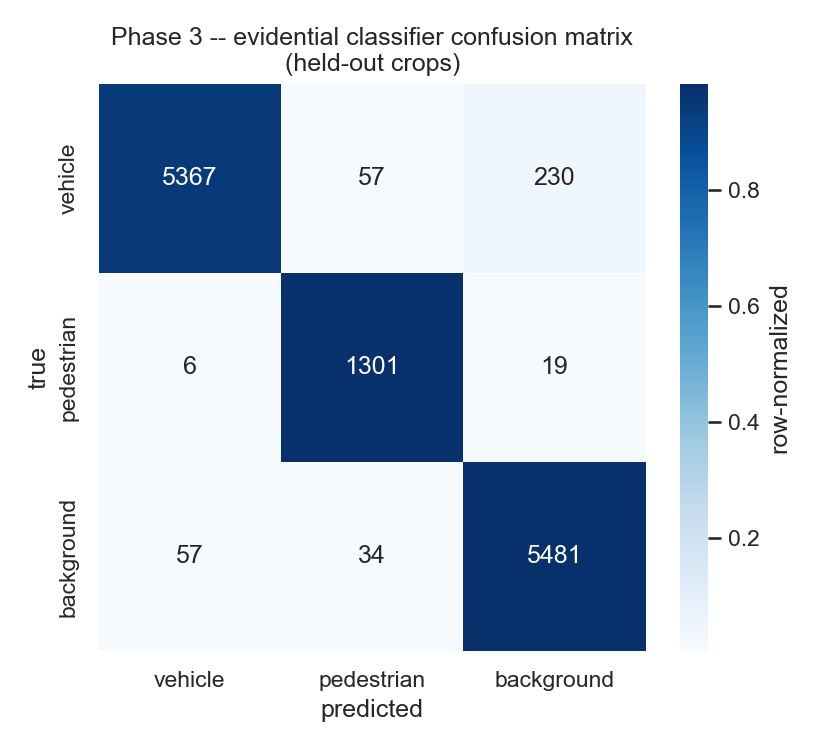
\includegraphics[width=0.9\linewidth]{figures/confusion_matrix.png}
\caption{Confusion matrix, evidential head, 12{,}552 held-out crops.}
\label{fig:confusion}
\end{figure}

Uncertainty is empirically calibrated: accuracy falls monotonically
from 99.4\% in the lowest-uncertainty bin to 63.0\% in the highest
(Figure~\ref{fig:calibration}), and the head is measurably more
uncertain on partially-visible crops (mean uncertainty 0.178) than on
clearly-visible ones (0.138). On an earlier dataset, before the deleted
fully-occluded ground truth described in Section~\ref{sec:dataset} was
restored, this calibration curve was flat. That was a data defect, not
a modelling one: the hard cases that should populate the
high-uncertainty bins had been discarded before training ever saw them.

\begin{figure}[htbp]
\centering
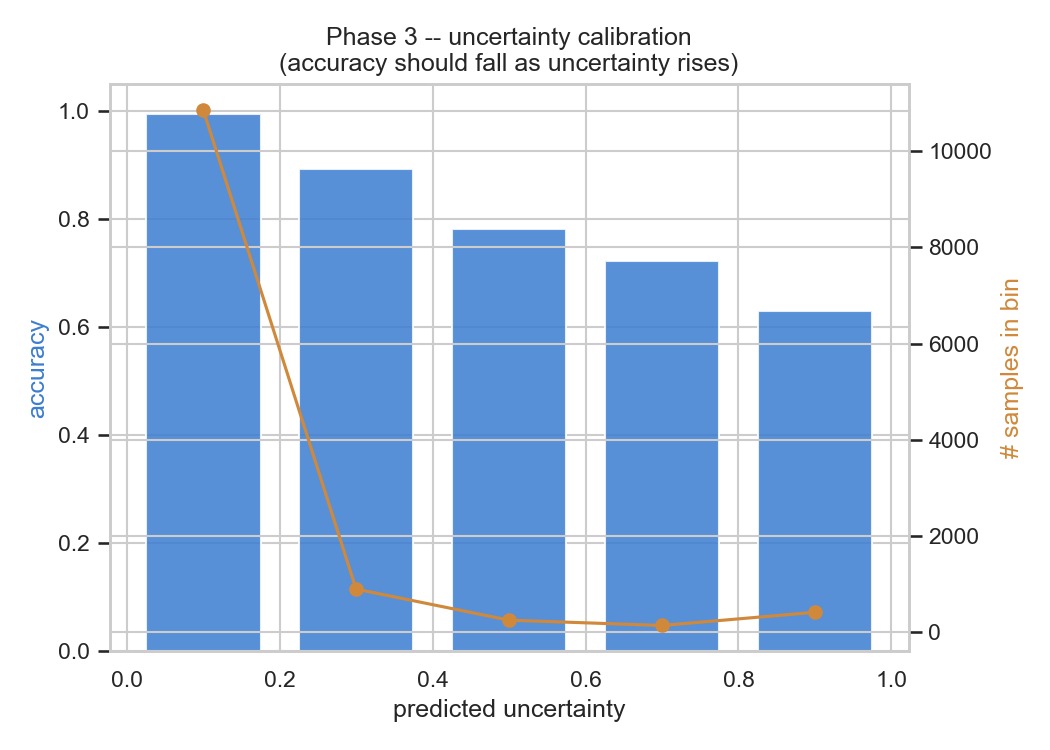
\includegraphics[width=0.9\linewidth]{figures/uncertainty_calibration.png}
\caption{Accuracy vs.\ self-reported uncertainty. Monotone decrease indicates calibration.}
\label{fig:calibration}
\end{figure}

\subsection{Occlusion Detector: A Ground-Truth Defect, Its Proof, and Its Correction}
\label{sec:occlusion-results}

The bird's-eye occlusion detector is evaluated against ground truth
computed from CARLA's own depth buffer via the \texttt{BevProjector}
class described in Section~\ref{sec:architecture}. During this
project, \texttt{BevProjector}'s vertical pixel projection was found to
contain a sign error: the formula mapped a ground point at forward
range 5~m to image row 106 of 600, near the top of the frame, i.e.\
sky, which is a physical impossibility for a level, forward-facing
camera. This was proven rather than just inferred, by cross-referencing
against a second, independently-implemented projection routine used for
two-dimensional amodal bounding boxes; once the sign was corrected, the
two agreed to $0.00$~px across every tested distance and lateral
offset. \texttt{BevProjector} was shared between the ground-truth
generator and, through a re-used class definition, was conceptually
adjacent to the runtime detector, so this defect was invisible to every
prior validation: ground truth and a structurally similar prediction
pathway shared the identical projection error, and comparing one
against the other tended to agree with itself regardless of what either
represented physically. Measured directly on freshly-collected frames,
the defective projection marked roughly 7--10\% of in-view cells
\textsc{occluded} in a typical urban frame. The corrected projection
marks 68--94\% \textsc{occluded} in the same kind of frame, because a
forward-facing, level camera under the defective formula was
frequently sampling sky rather than the ground plane.

The dataset was fully recollected against the corrected geometry.
Evaluated at the detector's then-existing default operating point,
recall collapsed from 0.629 (measured, invalidly, against the
defective ground truth) to \textbf{0.173} against the corrected ground
truth. A threshold sweep (Table~\ref{tab:sweep-old}) showed a maximum
achievable recall of only 0.479 at \emph{any} threshold. Precision
stayed high (0.978 at the sweep's most conservative point) because the
detector's own predictions had not changed; only the true count of
occluded cells to find had grown by an order of magnitude.

\begin{table}[htbp]
\caption{Threshold sweep, corrected ground truth, old disparity-quantile estimator}
\label{tab:sweep-old}
\centering
\begin{tabular}{@{}lrrr@{}}
\toprule
\texttt{shadow\_tolerance} & Precision & Recall & F1 \\
\midrule
0.02 (best F1, this estimator) & 0.842 & 0.479 & 0.610 \\
0.06 & 0.935 & 0.301 & 0.455 \\
0.12 (original default) & 0.978 & 0.194 & 0.323 \\
0.22 & 0.998 & 0.076 & 0.141 \\
0.40 & 1.000 & 0.011 & 0.022 \\
\bottomrule
\end{tabular}
\end{table}

A second, genuinely separate defect turned up next. The ground-profile
estimator fits ``clear ground'' as a low (0.30) quantile of disparity
within each range ring, but once a typical ring is 68--94\% truly
occluded, even its bottom-30th-percentile disparity is often estimated
from occluded, not clear, pixels: nearer objects read at \emph{higher}
disparity, so a majority-occluded ring drags even a low quantile
upward. That inflates the fitted ``ground'' level and suppresses recall
in exactly the dense scenes this system is meant for. Lowering the
quantile to 0.01 and jointly re-tuning the shadow-detection threshold
to 0.001, validated on a disjoint held-out sample with no frame overlap
with the tuning set to rule out overfitting, recovers precision 0.727,
recall \textbf{0.917}, F1 0.811 (Table~\ref{tab:sweep-new},
Figure~\ref{fig:sweep}). That is very nearly double the recall for a
precision cost of about 0.12, and it is the current, reported operating
point. The occlusion detector is no longer the weakest-performing
component of the system.

\begin{table}[htbp]
\caption{Ground-quantile / threshold co-tuning (held-out validated)}
\label{tab:sweep-new}
\centering
\begin{tabular}{@{}lrrrr@{}}
\toprule
Quantile / threshold & Prec. & Recall & F1 & Agree. \\
\midrule
0.30 / 0.02 (old) & 0.846 & 0.482 & 0.614 & 0.686 \\
\textbf{0.01 / 0.001 (new)} & \textbf{0.727} & \textbf{0.917} & \textbf{0.811} & \textbf{0.780} \\
\bottomrule
\end{tabular}
\end{table}

\begin{figure}[htbp]
\centering
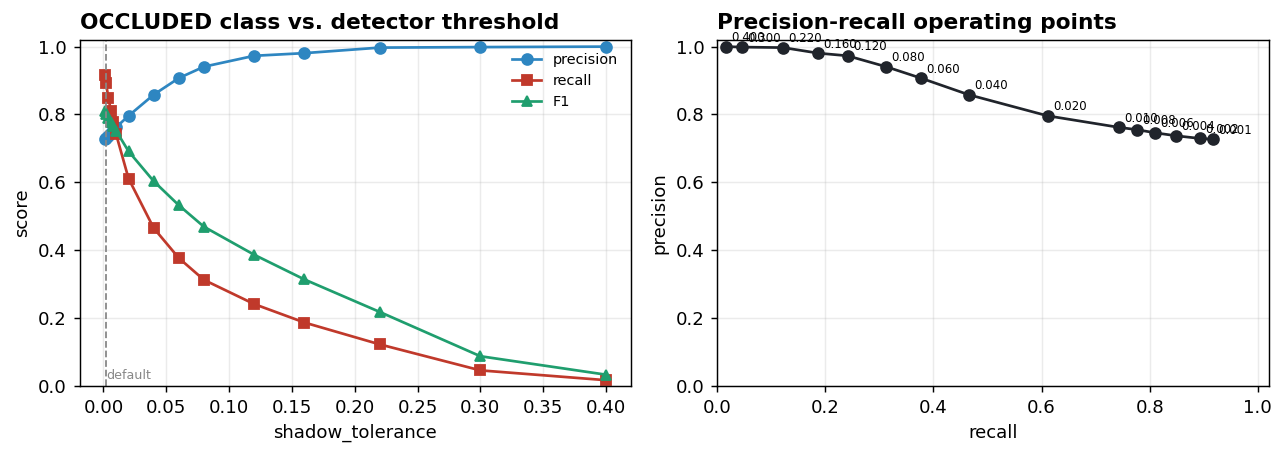
\includegraphics[width=0.9\linewidth]{figures/shadow_tolerance_sweep.png}
\caption{Precision/recall vs.\ shadow-detection threshold.}
\label{fig:sweep}
\end{figure}

\subsection{Sensor Fusion Ablation}

Camera-only, radar-only, and fused tracking configurations each confirm
tracks on a different subset of moving observations: 3{,}665; 2{,}491;
and 3{,}065, with only 845 tracked by all three. Comparing aggregate
means across these unequal, differently-difficult populations reverses
the correct conclusion. Unpaired, fusion looks worse than camera-only
on lateral-velocity error (0.963 vs.\ 0.857~m/s); paired on the 845
shared observations, fusion is clearly better (Table~\ref{tab:ablation}).
Radar is roughly $7\times$ more accurate than camera on forward
velocity, since Doppler measures the radial component directly, and
roughly $2.5\times$ worse on lateral velocity, since a target crossing
the ego's path has near-zero radial velocity: precisely the component
that decides a crossing outcome, and precisely the one radar cannot
see. Fusion improves on both single-sensor lateral-velocity results
(18\% better than camera-only, 60\% better than radar-only) because
lateral speed can be recovered as range (radar) times the rate of
change of bearing (camera), a quantity neither sensor alone supplies.

\begin{table}[htbp]
\caption{Sensor ablation, paired on 845 shared observations}
\label{tab:ablation}
\centering
\begin{tabular}{@{}lrrr@{}}
\toprule
Sensors & $v_{\text{lat}}$ MAE (m/s) & $v_{\text{fwd}}$ MAE (m/s) & Pos.\ err.\ (m) \\
\midrule
Camera only & 0.819 & 1.048 & 2.327 \\
Radar only & 1.683 & \textbf{0.155} & 2.457 \\
\textbf{Fused} & \textbf{0.672} & 0.199 & \textbf{2.032} \\
\bottomrule
\end{tabular}
\end{table}

\subsection{Crossing-Intent Prediction}

Fusion again dominates on the downstream prediction task
(Table~\ref{tab:intent}): AUC rises from 0.789 (camera-only) to 0.873
(fused), and F1 from 0.733 to 0.855, a 24-point recall improvement for
a 1.5-point precision cost relative to camera-only. Radar-only recall
is 0.018: it almost never predicts a crossing at all, which is Doppler
blindness to lateral motion showing up directly as a task metric.
Prediction degrades gracefully with visibility rather than failing
outright. Broken down by the tier at prediction time, AUC is 0.880 when
the target is clearly visible, 0.736 when partially visible, and
\textbf{0.635} even when the target is \emph{fully occluded} and the
track is coasting on dead reckoning alone. That is well above chance,
and it is the direct empirical payoff of the particle-filter
hidden-hazard mechanism described in Section~\ref{sec:architecture}.

\begin{table}[htbp]
\caption{Crossing-intent prediction by sensor configuration}
\label{tab:intent}
\centering
\begin{tabular}{@{}lrrrrr@{}}
\toprule
Sensors & $n$ & AUC & Prec. & Recall & F1 \\
\midrule
Camera only & 3{,}665 & 0.789 & 0.833 & 0.654 & 0.733 \\
Radar only & 2{,}491 & 0.743 & 1.000 & 0.018 & 0.035 \\
\textbf{Fused} & 3{,}065 & \textbf{0.873} & 0.818 & \textbf{0.896} & \textbf{0.855} \\
\bottomrule
\end{tabular}
\end{table}

Feeding classifier uncertainty into the crossing-intent covariance did
not move aggregate F1 or recall, and we report that as an honest null
result rather than a failed mechanism. The head is measurably more
uncertain on partial glimpses exactly as intended (mean uncertainty
0.178 vs.\ 0.138), but only 3.0\% of scored crops in this dataset are
partially visible, which leaves little for a caution mechanism to act
on in aggregate. This finding reproduced, at a similar magnitude,
across two independent data collections.

\subsection{Adversarial Robustness}

Table~\ref{tab:adversarial} summarises how the full pipeline and the
sensor health monitor respond to seven injected sensor faults plus a
geometric extrinsic-drift fault, replayed across 50 episodes. Every
camera fault is caught decisively: health drops from 0.93 to
0.05--0.06 under darkness, fog, blur, and sensor noise, and to 0.38
under a partially blocked lens. Radar dropout is caught too (0.82 to
0.40). Two faults are \emph{silent failures}: radar clutter raises
lateral-velocity error by 44\% and radar range bias costs 0.044 of
intent AUC, while the health monitor keeps reporting the radar as
healthy in both cases. That is, by design, the finding this evaluation
exists to surface. A pipeline that degrades while staying confident is
more dangerous than one that fails loudly, since nothing downstream has
any reason to discount its output.

\begin{table}[htbp]
\caption{Adversarial fault injection, 50 episodes}
\label{tab:adversarial}
\centering
\begin{tabular}{@{}lrrrl@{}}
\toprule
Condition & $v_{\text{lat}}$ MAE & Cam.\ h. & Rad.\ h. & Noticed \\
\midrule
Clean & 0.623 & 0.93 & 0.82 & --- \\
Darkness & 0.368 & 0.05 & 0.88 & Yes \\
Fog/blur/noise & 0.623 & 0.05--0.06 & 0.82 & Yes \\
Lens blocked & 0.508 & 0.38 & 0.86 & Yes \\
Radar dropout & 0.565 & 0.92 & 0.40 & Yes \\
\textbf{Radar clutter} & \textbf{0.900} & 0.93 & 0.91 & \textbf{No} \\
\textbf{Radar bias} & \textbf{0.813} & 0.93 & 0.82 & \textbf{No} \\
Extrinsic drift & 0.532 & 0.92 & 0.82 & No \\
\bottomrule
\end{tabular}
\end{table}

In the interest of reporting a negative result in full, we also
followed up on the radar-clutter case. The health monitor's existing
relative-scatter test (a Clark--Evans nearest-neighbour coherence index
compared against the sensor's own running median) turned out to catch
clutter only within a narrow window, roughly 200 frames, matched to the
length of its running baseline, after the fault onsets. A more
realistic, sustained clutter fault tested end to end over roughly
4{,}000 frames was not caught at all (health measured 0.90 both before
and after onset), because the running baseline accepts every frame
unconditionally, fault frames included, and a sustained fault
eventually overwrites its own reference. We implemented, measured, and
then reverted an attempted repair that excluded already-anomalous
samples from updating the baseline, because it dropped clean-condition
radar health from 0.82 to 0.48. Ordinary scene-to-scene variance in
this dataset (0.21--0.72 on the coherence index) is wider than the
clutter signal itself (0.383 clean vs.\ 0.499 injected), so an unlucky
early window locked in as ``normal'' and caused false alarms on
subsequent healthy driving that were worse than the gap the fix
targeted. Reverting a fix that measurably worsens the common case,
rather than keeping it because it improves the targeted metric, is
itself a result worth reporting.

Radar range bias is, by construction, undetectable by any
self-referential check once a tracking filter has converged: a constant
range offset is fully absorbed into the filter's converged state, so
its own residuals return to zero. A cross-sensor check that compares
radar range against an independent range estimate from a detection's
pixel height is correctly calibrated (mean offset 5.90~m against a
measured healthy-pairing calibration of 5.9~m, deviation 0.001~m over
5{,}805 pairs), but it needs roughly 2{,}500 paired observations for a
controlled false-positive rate. An earlier, 200-sample version of this
check looked correct in isolation but swung by up to $\pm16$~m between
episodes from association variance alone, and at that window size it
read radar health 0.54 on \emph{every} condition, including clean data
that never touches the radar: a uniform false alarm, not detection. At
2{,}500 samples this is resolved, but that sample count is more
exposure than a single 50-episode adversarial condition accumulates, so
\texttt{radar\_bias} still reads ``not noticed'' in
Table~\ref{tab:adversarial}. That is a property of this test's replay
length, not of the detector.

\subsection{Auxiliary Mechanisms}

The contradiction resolver's occlusion-conditioning is directly
measurable. For identical sensor readings, silence from both sensors,
the resolved posterior probability of a hazard is 0.009 in a
camera-confirmed-clear (\textsc{empty}) cell versus 0.152 in an
\textsc{occluded} cell (Figure~\ref{fig:contradiction}), a
17$\times$ difference in how the same observation gets read, which a
fixed-weight fusion rule cannot produce. The particle-filter
hidden-hazard tracker's multi-modality is likewise measurable rather
than asserted. On a synthetic occluded-crossing scenario, 20 hidden
frames (2.0~s) after a target disappears, 35\% of belief mass sits more
than 1~m to the left of the particle-cloud mean, 25\% more than 1~m to
the right, and only 41\% within 1~m of it (Figure~\ref{fig:particles}).
The mean position is itself a poor summary of where the hazard is
likely to be, which is exactly the failure mode a single Gaussian
filter cannot avoid.

\begin{figure}[htbp]
\centering
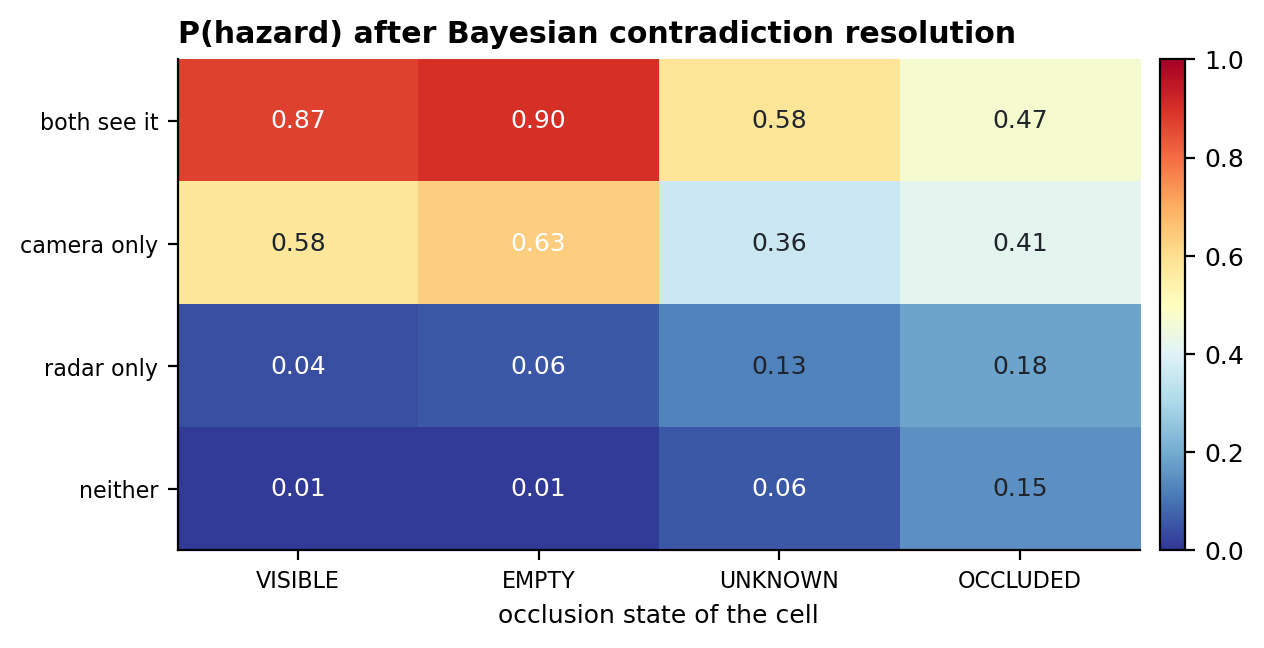
\includegraphics[width=0.9\linewidth]{figures/contradiction_matrix.png}
\caption{Posterior hazard probability by sensor-agreement case and occlusion state.}
\label{fig:contradiction}
\end{figure}

\begin{figure}[htbp]
\centering
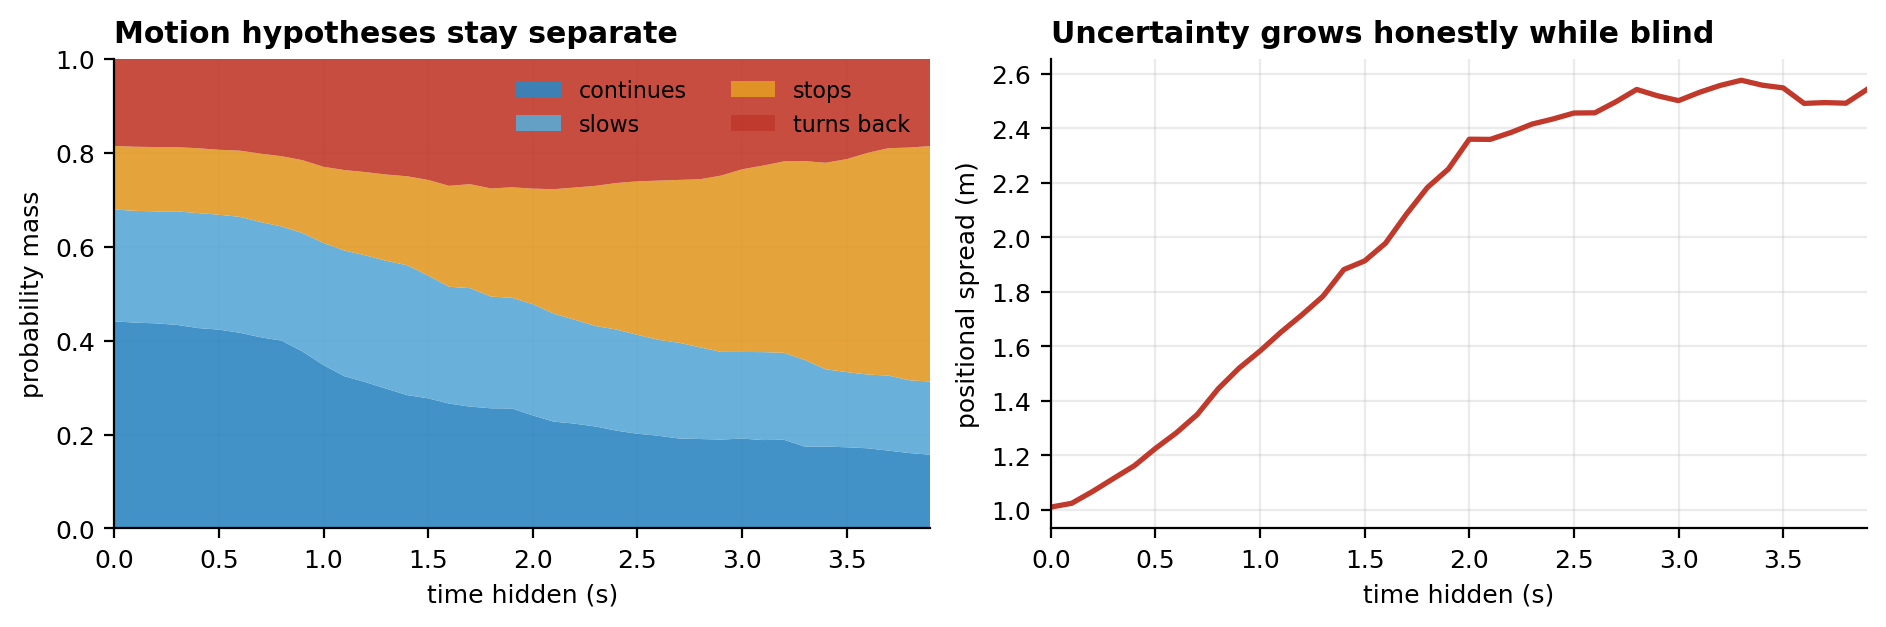
\includegraphics[width=0.9\linewidth]{figures/particle_modes.png}
\caption{Motion-hypothesis mass and positional spread while a hidden hazard is fully occluded.}
\label{fig:particles}
\end{figure}

\subsection{System Performance}

End-to-end measured throughput is 2--9~FPS (YOLOv8n, the evidential
head, MiDaS, the occlusion grid, and CARLA's own UE5.5 rendering all
sharing one consumer GPU), rising to 5.5--6.0~FPS once MiDaS refreshes
every third frame rather than every frame, since depth changes far more
slowly than radar returns do and the scene shifts well under one grid
cell between refreshes at city speed. Separately, as an operational
finding worth recording on its own, the CARLA~0.10.0 server was
measured to degrade by roughly $80\times$ over about 20~minutes of
continuous spawn/destroy activity (14.1~FPS fresh, 0.17~FPS after
sustained use, and this was independent of active traffic load), which
is why the final collection strategy used a fresh server per chunk.

\section{Discussion and Limitations}
\label{sec:discussion}

We report the following limitations plainly, in the same register as
the results above rather than as a closing formality.

\textbf{The CARLA~0.10.0 weather API does not work on this build.}
\texttt{get\_weather()} returns all-zero fields regardless of what is
set, and measured frame brightness does not move under an alternating
clear/night A/B test with a 40-tick settle window (three repetitions,
deltas of $-3.0$, $-3.1$, and $+0.3$ brightness points, where a genuine
night scene should differ by 100+ points). We re-confirmed this during
the project at higher (Epic) render quality, with manually constructed
weather parameters instead of named presets, and by searching for an
alternative, directly-manipulable sky/light actor; none exists on this
build. Adverse-condition robustness is therefore evaluated by applying
calibrated photometric degradations to captured clear-day frames rather
than by simulating weather natively. That is a weaker methodological
claim than genuine simulated weather, and we report it as such rather
than dress it up.

\textbf{The occlusion detector, while substantially improved, still
misses roughly 8\% of genuine occlusion} at its current operating
point. The precision/recall trade-off (0.727/0.917) was a deliberate
choice toward recall: a hidden-hazard signal is more useful catching
most real occlusion at moderate precision than catching half of it at
high precision, though a different downstream use case might reasonably
pick a different point on the same curve.

\textbf{Two sensor faults go undetected by the current health
monitor}: radar range bias present before the monitor begins observing,
and radar clutter sustained beyond its relative check's baseline
window. Both are properties of self-referential health monitoring in
general, rather than implementation defects specific to this system,
since a system cannot be inconsistent with a reference it has not yet
established, or that a long-enough fault has already absorbed into
itself. We report a genuine, measured attempt to fix the second one,
which made the common case worse and was reverted, rather than either
omitting the attempt or keeping a change that was not actually an
improvement.

\textbf{The evaluation is single-town and simulation-only.}
CARLA~0.10.0 ships a single usable town, so we make no claim about
generalisation across road geometries or building layouts, and no
claim about transfer to physical sensors: MiDaS on rendered imagery and
CARLA's idealised radar model are both more forgiving than a real
sensor stack is likely to be.

\section{Conclusion}
\label{sec:conclusion}

This paper presented a nine-component, occlusion-aware perception
architecture for autonomous driving that treats calibrated confidence,
explicit occlusion state, and multi-modal reasoning about hidden
hazards as first-class outputs rather than afterthoughts, and evaluated
it end to end in CARLA against a purpose-collected, 15{,}270-frame
dataset. The evidential classifier is accurate (96.2\%) and calibrated.
Camera--radar fusion measurably improves both velocity estimation
(18--60\% lateral error reduction, paired) and crossing-intent
prediction (F1 0.733 to 0.855) over either sensor alone, for the
physically grounded reason that camera and radar are blind to
complementary components of motion. The occlusion detector, after a
real ground-truth defect was found, proven, and corrected, and after a
further recall-limiting estimator defect was identified and fixed,
reaches 0.917 recall at 0.727 precision on a held-out validated
operating point. An explicit adversarial evaluation of the system's own
self-monitoring shows both what it catches, five of seven fault
classes, and, honestly, what it structurally cannot: sustained radar
clutter, and range bias present before observation begins, including a
fix attempt that was tried, measured to make the common case worse, and
reverted rather than kept. We think the methodological pattern
demonstrated throughout, validating ground truth independently rather
than trusting internal consistency, comparing sensor configurations on
paired rather than aggregate observations, and reporting null and
negative results in the same register as positive ones, matters at
least as much as any single measured number, and it should transfer
directly to other simulation-based, safety-relevant perception
research.

\section*{Acknowledgment}
The authors thank their project mentor for guidance throughout this work.

\begin{thebibliography}{00}

\bibitem{carla2017}
A.~Dosovitskiy, G.~Ros, F.~Codevilla, A.~L{\'o}pez, and V.~Koltun,
``CARLA: An open urban driving simulator,'' in \textit{Proc. 1st Annu.
Conf. Robot Learning (CoRL)}, 2017, pp.~1--16.

\bibitem{yolo2016}
J.~Redmon, S.~Divvala, R.~Girshick, and A.~Farhadi, ``You only look
once: Unified, real-time object detection,'' in \textit{Proc. IEEE
Conf. Comput. Vis. Pattern Recognit. (CVPR)}, 2016, pp.~779--788.

\bibitem{sensoy2018}
M.~Sensoy, L.~Kaplan, and M.~Kandemir, ``Evidential deep learning to
quantify classification uncertainty,'' in \textit{Advances in Neural
Information Processing Systems (NeurIPS)}, vol.~31, 2018.

\bibitem{welch1995}
G.~Welch and G.~Bishop, ``An introduction to the Kalman filter,''
Univ. North Carolina at Chapel Hill, Chapel Hill, NC, USA, Tech. Rep.
TR~95-041, 1995.

\bibitem{gordon1993}
N.~J. Gordon, D.~J. Salmond, and A.~F.~M. Smith, ``Novel approach to
nonlinear/non-Gaussian Bayesian state estimation,'' \textit{IEE Proc.
F (Radar and Signal Processing)}, vol.~140, no.~2, pp.~107--113, 1993.

\bibitem{clarkevans1954}
P.~J. Clark and F.~C. Evans, ``Distance to nearest neighbor as a
measure of spatial relationships in populations,'' \textit{Ecology},
vol.~35, no.~4, pp.~445--453, 1954.

\bibitem{ranftl2020}
R.~Ranftl, K.~Lasinger, D.~Hafner, K.~Schindler, and V.~Koltun,
``Towards robust monocular depth estimation: Mixing datasets for
zero-shot cross-dataset transfer,'' \textit{IEEE Trans. Pattern Anal.
Mach. Intell.}, vol.~44, no.~3, pp.~1623--1637, 2022.

\end{thebibliography}

\end{document}
